\documentclass[a4paper,10pt]{scrartcl}
\usepackage{physik-vorlesung}

\title{Physik Vorkurs}

\begin{document}

\maketitle

\tableofcontents
\newpage
\section{Grundlagen}
\subsection{Was ist Physik}
\begin{seg}{(Versuch einer Definition)}
 Physik ist eine \emph{Naturwissenschaft}, die sich mit der \emph{rationalen Beschreibung} von Naturerscheinungen mit der Untersuchung der \emph{Ursachen und Wirkungen}.
\end{seg}
\begin{seg}{Grundprinzipien}

\begin{description}
 \item[WIE?] Naturwissenschaft $\longrightarrow$ Methode
 \item[WAS?] rationale Beschreibung $\longrightarrow$ Unterteilung
 \item[WARUM?] Ursachen und Wirkungen $\longrightarrow$ Zusammenhang der Gesetze, Reproduzierbarkeit
\end{description}
\end{seg}

\subsubsection{Gegenstand der Physik}
\begin{seg}{klassische Unterteilung:} 
 Mechanik, E-Lehre, Thermodynamik, etc.
\end{seg}

\begin{ex}[Blitz]
 \begin{itemize}
  \item Funkentladung: $20000 A$
  \item Erhitzung der Luft: $T \approx 30000 K$
  \item Schall: Druck
  \item B-Feld
 \end{itemize}
\end{ex}

\begin{enumerate}
 \item Behandle jedes Phänomen als unabhängig
 \item Zusammenhänge: der hypothetisch-deduktive Ansatz
\begin{enumerate}
 \item Beschreibung
 \item Hypothesenfindung
 \item Deduktion
 \item Experiment
\end{enumerate}

\end{enumerate}

\begin{merke}
 Dieses Verfahren hat ausschließlich eine Provisorische Gültigkeit und liegt in der Regel einem Veränderungsprozess zu Grunde.
\end{merke}

\begin{ex} Newtonsche Gravitationsgesetze

 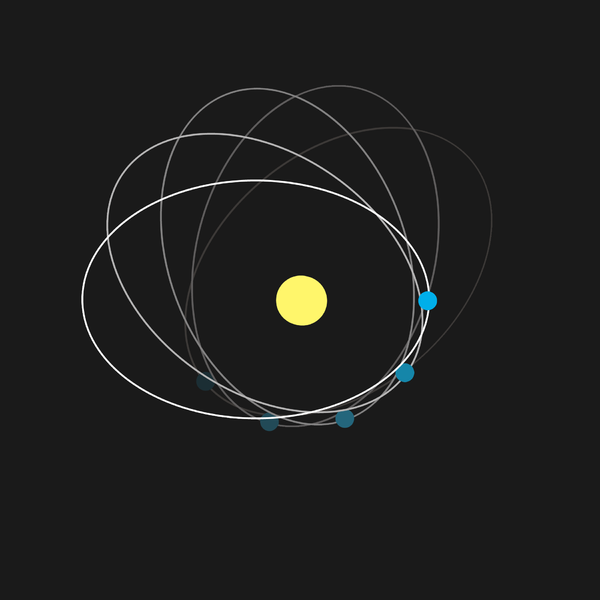
\includegraphics[scale=0.1]{apsidendrehung.png}
\emph{Apsiden- oder Periheldrehung}

Unter einer Apsidendrehung versteht man die Drehung der Ellipsenbahn eines Planeten, dieser lässt sich teilweise durch die Newtonsche Gravitationsgesetze bestimmen zu:

\begin{tabular}{l c r}
Venus & $\rightarrow$ & $280''$ \\
Jupiter & $\rightarrow$ & $150''$ \\
Planeten & $ \rightarrow$ & $100''$ \\
Beschreibung & $\rightarrow$ & $571,91''$
\end{tabular}

Es ergibt sich eine Diskrepanz von $43''$.  Unter Einbeziehung der \emph{allgemeinen Relativitätstheorie} verbleibt eine Diskrepanz von $42''$.  Die Newtonsche Gravitationsgesetze reichen nicht aus, um die \emph{Anomalie} zu beschreiben.
\end{ex}

\subsection{Physikalische Gesetze}
Eine \emph{physikalische Größe}  ist eine quantitative bestimmte Eigenschaft eines  physikalischen Objekts.

Sie besitzt einige charakteristische Eigenschaften:
\begin{itemize}
 \item Maßvorschrift: 
\subitem $\mapsto$ direkt [Bsp.: Meterstab]
\subitem $\mapsto$ geeichtes Instrument [Bsp.: Federwage]
\subitem $\mapsto$ indirekt [Bsp.: Flächeninhalt Dreieck] 
 \item Messaparatur
 \item Einheit:  $G=\underbrace{\{G\}}_{\text{Maßzahl}}\underbrace{[G]}_{\text{Einheit}}=n\cdot U_G$
\end{itemize}
\begin{ex} Grundgrößen der Mechanik
\begin{table}[h]
\begin{tabular}{l c c l}
 Größe:  &   Anwendung: & Einheit & Messaparatur\\
 1) Länge: &  Raummessung & \textbf{m} & Meterstab\\
 2) Zeit: & Abfolge von Ereignissen & \textbf{s} & Uhr\\
 3) Masse: & Eigenschaft der Materie & \textbf{kg} & Waage
\end{tabular}
\end{table}

Länge und Zeit bilden hierbei die \emph{Kinematik}.  Länge, Zeit und Masse stellen die \emph{Dynamik} dar.
\end{ex}

\subsubsection{Dimension und Einheit}
$G=L^\alpha M^\beta T^{\gamma}$, $\alpha$, $\beta$ und $\gamma$ bezeichnet man als die \emph{Dimensionen} der Grundgrößen der Mechanik $L, M, T$.
\begin{note}
 In der Regel arbeitet man mit ganzzahligen Dimensionen.
\end{note}

\begin{ex}

\begin{itemize}
 \item \emph{Fläche} $[A]=[L^2 M^0 T^0]=[L^2]$
 \item \emph{Volumen} $[V]=[L^3M^0T^0]=[L^3]$
 \item \emph{Geschwindigkeit} $[v]=[L^1M^0T^{-1}]=[L^1 T^{-1}]$
\end{itemize}
Hiermit stellen \emph{Fläche} und \emph{Volumen} kinematische und die \emph{Geschwindigkeit} dynamische Größen dar.
\end{ex}
\newpage  
\begin{seg}{Methode: Umrechnung}
 Seien $G=n_1\cdot U_{1L}^\alpha U_{1M}^\beta U_{1T}^\gamma$ und $G=n_2\cdot U_{2L}^\alpha U_{2M}^\beta U_{2T}^\gamma$ Darstellungen von $G$.
 \[
  \implies n_2=n_1 \cdot \left ( \frac{U_{1L}}{U_{2L}} \right )^\alpha \left ( \frac{U_{1M}}{U_{2M}} \right )^\beta \left ( \frac{U_{1T}}{U_{2T}} \right )^\gamma
 \]
\end{seg}
\begin{ex}
 Bestimmung des Flächeninhalts eines Rechtecks der Größe $10 \text{cm} \times 1\txt{cm}$.  Der Inhalt ergibt sich also zu $A=10\text{cm}\cdot 1 \text{cm}=10\txt{cm}^2=x\txt{m}^2$.  Berechne $x$.
\[
 x=10 \left ( \frac{1 \txt{cm}}{1 \txt{m}} \right ) = 10 \left ( \frac{1 \txt{cm}}{100 \txt{cm}} \right )=0,001
\]

\end{ex}

\subsubsection{Messfehler}
\begin{enumerate}
 \item Systematische: $T=\omega \pm \sigma$
 \item statischtische Fehler:
 \begin{itemize}
  \item $N$ Messungen
  \item Quadratische Abweichung: $A=\sum_{i=1}^{N}(x-x_i)^2$
\subitem $\mapsto$ Suche Minimum:
\[
 \frac{dA}{dx} \mid_{x=\tilde x}=2 \sum_{i=1}^N(x-x_i) \mid_{x=\tilde x}\stackrel{!}{=}0
\]
\[
  \implies \sum_{i=1}^N x_i=\sum_{i=1}^N \tilde x=N\tilde x \implies \tilde x=\frac{1}{N}  \sum_{i=1}^N x_i
\]


 \end{itemize}

\end{enumerate}

\section{Mechanik eines Massenpunktes}

\subsection{eindimensionale Bewegung}


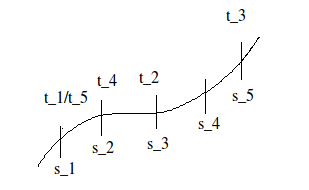
\includegraphics[scale=0.5]{pic1.png}

Eine eindimensionale Bewegung lässt sich auf verschiedene Arten darstellen.  Hier einige Beispiele:


\begin{enumerate}
 \item Ort-Zeit-Tabelle

\begin{tabular}{l|c|c|c|c|c|}
 $t[\text{s}]$ & 1 & 2& 3 & 4 & 5\\
 $s[\text{m}]$ & 1 & 3& 5 & 2 & 1
\end{tabular}

\item Ortsfunktion: $\qquad s=s(t)$

\item Ort-Zeit Diagramm

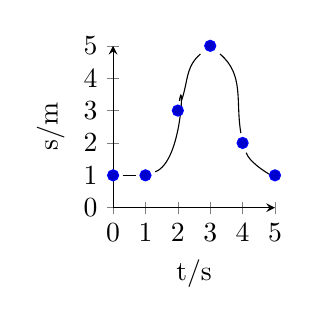
\begin{tikzpicture}
      \begin{axis}
       [
         axis x line  = bottom,
         axis y line  = left,
         width        = 0.3\textwidth,
         height       = 0.3\textwidth,          % Adjusted
         ymax         = 5,
         ymin         = 0,
         ytick        = {0,1,...,5},
         xmax         = 5,
         xmin         = 0,
         xlabel       = t/s,
         ylabel       = s/m,
         xtick        = {0, 1, ..., 5},
	 mark        = *,
	 color       = black,
         fill        = black,
	 only marks
       ]
       \addplot coordinates {
        ( 0, 1 )
	( 1, 1 )
	( 2, 3 )
	( 3, 5 )
	( 4, 2 )
	( 5 , 1 )
	};
        \node (A) at (axis cs:0,1){};
	\node (B) at (axis cs:1,1){};
	\node (C) at (axis cs:2,3){};
	\node (D) at (axis cs:3,5){};
	\node (E) at (axis cs:4,2){};
	\node (F) at (axis cs:5,1){};
	\draw[-](A) to (B);
	\draw[-](B) to [out=20, in=81] (C);
	\draw[-](C) to [out=70, in=220] (D);
	\draw[-](D) to [out=-40, in=100] (E);
	\draw[-](E) to [out=-70, in=-30] (F);
       
       

      \end{axis}
   \end{tikzpicture}
\end{enumerate}

\begin{itemize}
 \item mittlere Geschwindigkeit
\[
 \_v= \frac{s(t_2)-s(t_1)}{t_2-t_1} L^1 T^{-1} \frac{\text{m}}{\text{s}}
\]
\[
 \implies [s(t_2)=\_v (t_2-t_1)+s(t_1) 
\]
Man nennt diese Gleichung auch das \emph{Weg-Zeit-Gesetz}
\end{itemize}
\begin{note}
\[
 \_v_{t_1t_2}=\frac{(3-1)\text{m}}{(2-1)\text{s}}=2 \frac{m}{s}>0
\]
\[
 \_v_{t_2,t_4}=
\]
\[
 \_v_{t_1,t_5}=
\]

\[ 
 \_v^{\text{Reise}}_{t_2t_4}=\frac{5 \text{m}}{2\text{s}}=2,5 \frac{\text{m}}{\txt{s}}
\]

\end{note}

\subsubsection{Momentangeschwindigkeit}
\[
 \exists s(t)\forall t: v(t)=\lim\limits_{\Delta t \rightarrow \infty} \frac{\Delta s}{\Delta t}
\]
Die \emph{Momentangeschwindigkeit} $v(t)$ kann dabei positiv, negativ oder null werden.

Fallunterscheidung:
\begin{enumerate}
 \item $v(t)>0: \Delta s >0$, daher $s(t+\Delta t)>s(t)$
 \item $ v(t)<0: \Delta s<0$, daher $s(t+\Delta t)<s(t)$
 \item $ v(t)=0: \Delta s=0$, daher $s(t+\Delta t)=s(t)$
\end{enumerate}
 

\subsection{dreidimensionale Bewegung}

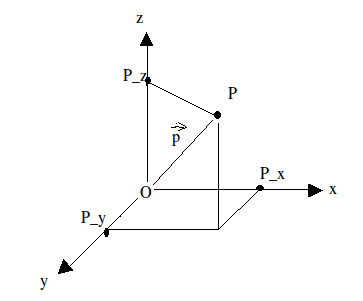
\includegraphics[scale=0.5]{pic2.png}

Die obige Darstellung entspricht der \emph{kartesichen} Darstellung eines Punkts.

Ort-Zeit-Tabelle:
\begin{table}[h]
 \begin{tabular}{c|c|c|c|c|c}
  $t[\txt{s}]$ & $ t_1$ & $\ldots$ & $t_x$ & $\ldots$ & $t_N$\\
  $x[m]$ & $x_1$ & $\ldots $ & $x_x$ & \ldots & $x_N$ \\
 $y[m]$ & $y_1$ & $\ldots $ & $y_x$ & \ldots & $y_N$ \\
$z[m]$ & $z_1$ & $\ldots $ & $z_x$ & \ldots & $z_N$ \\ 
 \end{tabular}

\end{table}

Ortsfunktionen: $x=x(t), \qquad y=y(t), z=z(t)$

\subsection{Skalare mit Vektoren}
\begin{itemize}
 \item Skalare Größen: Temperatur
 \item Vektoren
 \begin{enumerate}
  \item Betrag
  \item Richtung
  \item Sinn
 \end{enumerate}

\begin{note}
 Ein Skalare Größe kennzeichnet sich durch Invarianz bei Drehung, Verschiebung...
\end{note}

\item Komponentendarstellung

Wir unterteilen kartesische Koordinatensysteme (Achsen stehen senkrecht zueinander)...  Dann definiert man Komponentenvektoren $e_x$, $e_y$, $e_z$.\\
\[
 \vec a=\begin{pmatrix}a_x\\a_y\\a_z\end{pmatrix}=a_x e_x+a_y e_y+a_z e_z
\]

Der Betrag definiert sich zu $ |\vec a|=\sqrt{a_x^2+a_y^2+a_z^2} $
\end{itemize}
\subsubsection{Elementare Operationen}
\begin{itemize}
\item Multiplikation mit Skalar: 
\[
 \alpha \cdot \vec a=\begin{pmatrix} \alpha a_x \\ \alpha a_y \\ \alpha a_z \end{pmatrix}
\]

Für $\alpha>0$ ergibt sich eine Zerrung des Vektors.  Für $\alpha<0$ erfolgt außerdem eine Spiegelung des Vektors mit anschließlicher Zerrung mit $|\alpha|>0$.  Für $\alpha=0$ wird der Vektor auf den Nullvektor abgebildet.

\item Addition/Subtraktion:

\[
 \vec a + \vec b = \begin{pmatrix} a_x+b_x \\ a_y+b_y\\ a_z+b_z \end{pmatrix}
\]
\begin{seg}{Geometrische Interpretation der Addition von Vektoren}
 Die Addition von Vektoren ist gerade der Vektor, der entsteht, wenn ein Punkt hintereinander mittels der Vektoren verschoben wird. Der daraus entstehende Verbindungsvektor entspricht dann der Addition der Vektoren.
\end{seg}


\item Skalarprodukt:
\[
 \vec a \cdot \vec b= |\vec a| |\vec b| \cos(\alpha)
\]
Das Skalarprodukt besitzt einige wichtige Eigenschaften:
\begin{itemize}
 \item $\vec a \cdot \vec b = \vec b \cdot \vec a$
 \item $\vec a \orth \vec b \equiv \vec a \cdot \vec b =0$
 \item $|a|=\sqrt{\vec a \cdot \vec a}$
\end{itemize}
\item Kreuzprodukt

Das Kreuzprodukt zwischen zwei Vektoren ist definitiert als $\vec a \times \vec b = \vec c$ mit $|\vec c|= |\vec a| |\vec b| \sin(\alpha)$.

Die geometrische Interpretation ist gerade, dass der Vektor senkrecht zu $\vec a$ und $\vec b$ steht und von der Länge $|\vec c|$ ist.

wichtige Eigenschaften des Kreuzprodukts:
\begin{itemize}
\item $\vec a \times \vec b = \vec c$
\item $\vec b \times \vec a= -\vec a \times$ 
\item $e_x \times e_y=e_z, \qquad e_y\times e_z=e_x, \qquad e_z\times e_x=e_y$
\end{itemize}

Die Komponentendarstellung führt zu:
\[
 \vec c = e_x (a_y b_z-a_zb_y)+e_y(a_zb_x-a_xb_z)+e_z(a_xb_y-a_yb_x)
\]

Es gibt verschiedene Methode um sich dies zu merken. Wir verweisen hier auf externe Literatur.

\end{itemize}
\subsection{Kinematik}
\subsubsection{Geschwindigkeitsvektor}
\fixme{Zeichnung}
\begin{itemize}
 \item mittlere Geschwindigkeit
 \[
 \vec v_m= \frac{\vec s(t_1)- \vec s(t_2)}{t_1-t_2}=??
\]
\item Momentangeschwindigkeit
\[
 \vec v(t)=\lim\limits_{\Delta t \rightarrow 0}= \frac {\vec s (t+\Delta t)-\vec s (t)}{\Delta t} = 
\]
\fixme[Differential von s nach t und punktweise differentiation.
\item  $\frac{d |\vec s|}{dt}=\frac{d}{dt} \sqrt{\vec s \vec s}
=\frac 1 2 \frac 1 {\sqrt{\vec s \vec s }}  [  \frac{d\vec r}{dt}  
\cdot \vec r + \vec r \cdot \frac{d\vec r}{dt}  ]
=\frac{\vec r \vec v}{|\vec r|}\stackrel{!}= 0 \implies \vec r \orth \vec v$
\end{itemize}
\[
 \vec v_m= \frac{\vec s(t_1)- \vec s(t_2)}{t_1-t_2}=??
\]

\subsubsection{Beschleunigungsvektor}

\[
 \vec a (t)=\lim\limits_{\Delta t} \frac{\vec v(t+\Delta t)-\vec v(t)}{\Delta t}
\]
\fixme[Differential und Punktschreibweise wie auch Punktschreibweise der Komponenten]

\begin{seg}{Zerlegung von $\vec a$}
\[
  \vec a = \frac{d}{dt} (v \hat T)=\underbrace{\frac{dv}{dt} \hat T}_{\txt{Tangentialkomponente: }\vec \alpha_T}+ 
 \underbrace{\vec v \frac{d\hat T}{dt}}_{\txt{Normalkomponente: }\vec a_N}
=\vec v \hat T + \underbrace{\alpha}_{\frac{\vec v^2}{R}} \cdot \hat N
 \]

Nebenrechnung:
 \[
 \frac{d\hat T}{dt}=0 \rightarrow \frac{{d\hat{T}}^2}{{dt}}= 2 \hat T\cdot \frac{d\hat T}{dt} ~ \hat N
 \]

\fixme[grafische Darstellung der Komponente]

\fixme[Diagramm: Klassifizierung der Beschleunigung]

\begin{ex}[schräger Wurf]
 blabla
\end{ex}


\end{seg}






\section{Elektrizität und Stromlehre}

\section{Thermodynamik}





\end{document}